\documentclass{article}

%%%%%%%%%%%%%%%%%%%%%%%%%%%%%%%%%%%%%%%%%%%%%%%%%%%%%%%%%%%%%%%%%%%%%%%%%%%%%%%
%% Packages

\usepackage{PRIMEarxiv}
\usepackage[utf8]{inputenc} % allow utf-8 input
\usepackage[T1]{fontenc}    % use 8-bit T1 fonts
\usepackage{hyperref}       % hyperlinks
\usepackage{url}            % simple URL typesetting
\usepackage{booktabs}       % professional-quality tables
\usepackage{amsfonts}       % blackboard math symbols
\usepackage{nicefrac}       % compact symbols for 1/2, etc.
\usepackage{microtype}      % microtypography
\usepackage{lipsum}
\usepackage{fancyhdr}       % header
\usepackage{graphicx}       % graphics
\usepackage{float}
\usepackage{amsfonts}
\graphicspath{{media/}}     % organize your images and other figures under media/ folder
\usepackage[dvipsnames]{xcolor}
\usepackage{xparse}
%%%%%%%%%%%%%%%%%%%%%%%%%%%%%%%%%%%%%%%%%%%%%%%%%%%%%%%%%%%%%%%%%%%%%%%%%%%%%%%
%% Custom Commands

\newcommand{\toolstyling}[1]{#1}
\newcommand{\rawnet}{\toolstyling{RawNet2}}

\newcommand{\Mel}{\toolstyling{MelGAN}}
\newcommand{\PWG}{\toolstyling{PWG}}
\newcommand{\MBMel}{\toolstyling{MB-MelGAN}}
\newcommand{\FBMel}{\toolstyling{FB-MelGAN}}
\newcommand{\hifi}{\toolstyling{HiFi-GAN}}
\newcommand{\wav}{\toolstyling{WaveGlow}}

\newcommand{\diffw}{\toolstyling{DiffWave}}
\newcommand{\FTTS}{\toolstyling{TTS}}

\newcommand{\overbar}[1]{\mkern 1.5mu\overline{\mkern-1.5mu#1\mkern-1.5mu}\mkern 1.5mu}

%%%%%%%%%%%%%%%%%%%%%%%%%%%%%%%%%%%%%%%%%%%%%%%%%%%%%%%%%%%%%%%%%%%%%%%%%%%%%%%
%% Header
\pagestyle{fancy}
\thispagestyle{empty}
\rhead{ \textit{ }} 

% Update your Headers here
% \fancyhead[LO]{Running Title for Header}
% \fancyhead[RE]{Firstauthor and Secondauthor} % Firstauthor et al. if more than 2 - must use \documentclass[twoside]{article}

%%%%%%%%%%%%%%%%%%%%%%%%%%%%%%%%%%%%%%%%%%%%%%%%%%%%%%%%%%%%%%%%%%%%%%%%%%%%%%%
%% Title
\title{Audio DeepFake Detection\thanks{\textit{A Course Project for SUTD 50.039 Theory and Practice of Deep Learning (2022 Spring)}}
}

%%%%%%%%%%%%%%%%%%%%%%%%%%%%%%%%%%%%%%%%%%%%%%%%%%%%%%%%%%%%%%%%%%%%%%%%%%%%%%%
%% Authors
\author{
    Mark He Huang\thanks{These authors have contributed equally.} \hfill Peiyuan Zhang\footnotemark[2] \hfill James Raphael Tiovalen\footnotemark[2] \hfill Madhumitha Balaji\footnotemark[2]\\
    Information Systems Technology and Design (ISTD) Pillar \\
    Singapore University of Technology and Design \\
    Singapore, Singapore\\
    \texttt{\{he\_huang, peiyuan\_zhuang, james\_raphael, madhumitha\_balaji\}@mymail.sutd.edu.sg} \\
    \And
    Shyam Sridhar\footnotemark[2] \\
    Engineering Systems and Design (ESD) Pillar \\
    Singapore University of Technology and Design \\
    Singapore, Singapore\\
    \texttt{shyam\_sridhar@mymail.sutd.edu.sg} \\
}

%%%%%%%%%%%%%%%%%%%%%%%%%%%%%%%%%%%%%%%%%%%%%%%%%%%%%%%%%%%%%%%%%%%%%%%%%%%%%%%
%% Begin Document
\begin{document}
\maketitle

%%%%%%%%%%%%%%%%%%%%%%%%%%%%%%%%%%%%%%%%%%%%%%%%%%%%%%%%%%%%%%%%%%%%%%%%%%%%%%%
%% Abstract

% \begin{abstract}
% \lipsum[1]
% \end{abstract}
% \keywords{DeepFake Detection \and Synthetic Voice \and Deep Learning}

%%%%%%%%%%%%%%%%%%%%%%%%%%%%%%%%%%%%%%%%%%%%%%%%%%%%%%%%%%%%%%%%%%%%%%%%%%%%%%%
%% Introduction
\section{Introduction}

DeepFake audio refer to those that are fabricated and are underpinned by deep neural networks (DNN) that learn the movements of sound recordings to the extent that they can produce realistic-sounding fake audio. They are generally used to imitate people's voices. While they could, at times, be amusing, such techniques can be misused to spread misinformation which can lead to detrimental consequences. Some of the ways in which DeepFake techniques can be exploited include online harassment, influencing political movements, and people impersonation. For example, audio DeepFake coupled with image DeepFake might potentially be used as a tool for information warfare between Russia and Ukraine\cite{Zelensky}. Therefore, there has been tremendous attention devoted to designing and implementing realistic audio DeepFake detection systems in recent years. In this project, we focus on distinguishing DeepFake audio that are generated by various state-of-the-art GAN-based DNN apart from the real ones. We explore different sequential modelling architectures as well as different base features for DeepFake audio detection. We release code and results on GitHub: \url{https://github.com/MarkHershey/AudioDeepFakeDetection}

%%%%%%%%%%%%%%%%%%%%%%%%%%%%%%%%%%%%%%%%%%%%%%%%%%%%%%%%%%%%%%%%%%%%%%%%%%%%%%%
%% Related Works
\section{Related Works}

\textbf{Audio DeepFake detection.}
Plenty of models was proposed to filter out fake audio from the real ones. \cite{Subra2020Learning} tries to provide a more fine-grained supervision signal by having two classification blocks. The first is to predict the binary fake or real label, while the second tries to output the type of audio synthesis technique used to generate the fake audio. Instead of training a model from scratch, \cite{Wang2020DeepSonar} proposes to use the hidden layer neuron activation map from an existing speaker recognition (SR) model as the feature representation of an audio file. They then feed this representation to a lightweight classifier to output the final prediction. Meanwhile, \cite{shallowcnn2019} proposes to utilize a shallow CNN-based approach in differentiating real voice audio from synthetic ones. \cite{Wu2022SelfAttention} proposes a brand new framework for locating the fake regions in the overall input audio. They do so by equipping the fake span discovery strategy with a self-attention mechanism in order to enhance their quality of detection. \cite{JungReplay2019} aims to provide a solution to replay attacks, where an attacker acquires a target speaker’s voice using a recording device and then replays using a playback device. The attacker does this using different combinations of replay and playback devices with background environments. In order to defend against this class of attacks, the authors propose using an end-to-end DNN without knowledge-based intervention. \cite{2020res2net} also proposes another method to conduct replay and speech synthesis detection via the usage of two blocks: a Res2Net block and a squeeze-and-excitation block.

\textbf{Audio Processing.} Digital audio signals are records of the original sound waves at a certain sample frequency, i.e. sampling rate. Traditional statistical models \cite{xu2004hmm} usually take pre-processed audio features, such as the Mel Frequency Cepstral Coefficients (MFCC) or the Linear Frequency Cepstral Coefficients (LFCC) as the model input. MFCC is one of the most commonly used audio features because its frequency bands are designed to be close to the human auditory system. To derive the MFCC features from waveform signals, we first transform the waveform signal into a Mel-scaled spectrogram, then followed by taking an logarithm and applying a discrete cosine transform as shown in Equation \ref{equation:mfcc}. LFCC is similar to MFCC, but it uses a linear scale filter, which will result in more of the high frequency signal being retained compared to the MFCC feature. Deep learning-based models take in various kind of audio inputs, including raw waveform, spectrogram, Mel-spectrogram, MFCC/LFCC, etc. In addition, Double Delta augmentation are often used on top of MFCC/LFCC, which takes the first and second derivatives as shown by Equation \ref{equation:delta} to further enhance temporal representation.

\begin{equation}\label{equation:mfcc}
    c(t, r) = \sum_{s=0}^{S-1}\log\big[X_{\mathrm{mel}}(t,s)\big] \cdot \text{cos}\bigg[\frac{\pi \cdot r\cdot(s+0.5)}{S}\bigg] \quad \forall  r = 0,\dots, R-1,
\end{equation}
\begin{equation}\label{equation:delta}
    d(t) = \frac{\sum_{n=1}^N n\cdot\big[c\,(t+n)-c\,(t-n)\big]}{2\cdot\sum_{n=1}^N n^2} \quad \forall  t = 0,\dots, T-1,
\end{equation}

In our work, we experiment with various model architectures, equipped with different audio features, to compare their performance. All MFCC or LFCC features used in our project are augmented using Double Delta.

%%%%%%%%%%%%%%%%%%%%%%%%%%%%%%%%%%%%%%%%%%%%%%%%%%%%%%%%%%%%%%%%%%%%%%%%%%%%%%%
%% Dataset
\section{Dataset}

For the source of real audio data, we use LJSpeech \cite{ljspeech17}, which is a high-quality human speech dataset consisting of 13,100 short audio clips (ranging from approximately 1-10 seconds, 24 hours in total) of a single female speaker reading passages from 7 non-fiction books. For the source of deep fake audio data, we use WaveFake \cite{frank2021wavefake}, a dataset based on LJSpeech \cite{ljspeech17}, introduced in 2021 at NeurIPS. It consists of 117,985 synthetic audio clips (196 hours in total) generated by six different deep learning-based generative network architectures (i.e., \textbf{\Mel{}} \cite{kumar2019melgan}, \textbf{Parallel WaveGAN (\PWG{})} \cite{van2016wavenet}, \textbf{Multi-band MelGAN (\MBMel{})} \cite{frank2021wavefake}, \textbf{Full-band MelGAN (\FBMel{})} \cite{frank2021wavefake}, \textbf{HiFi-GAN (\hifi{})} \cite{kong2020hifi}, and \textbf{WaveGlow} \cite{kingma2018glow}). Each of the six deep neural networks generates 13,100 audio clips corresponding to the real audio clips in LJSpeech \cite{ljspeech17}.

%%%%%%%%%%%%%%%%%%%%%%%%%%%%%%%%%%%%%%%%%%%%%%%%%%%%%%%%%%%%%%%%%%%%%%%%%%%%%%%
%% Methods
\section{Methods}

\subsection{Gaussian Mixture Model}

Motivated by previous works such as \cite{spoofingdetection2020, AlluriV19-0, Bhushan2019}, we developed a GMM based approach to deepfake audio detection. Specifically, our classifier is composed of 2 Gaussian Mixture Models that were trained individually on real and generated audio samples. Each model is composed of 128 single Gaussian models. The Gaussian distribution is chosen here as the choice of the probability distribution for the mixture model, given its unique mathematical properties and its good computational performance.

The two models used the MFCC features that we extracted from the audio files as inputs. The final classification is made according to the likelihood function:
\begin{equation}
    f(x) = \log{p(x|\theta_r)} - \log{p(x|\theta_g)}
\end{equation}
where $\theta_r$ and $\theta_g$ are the Gaussian parameters for the real and generated audio distributions respectfully with $x$ being the input MFCC feature.

\subsection{Vanilla Recurrent Neural Network}

Audio is by nature a kind of sequential data, in which the waveform manifests different frequencies and amplitudes in different timestamps. Vanilla Recurrent Neural Network (RNN) is the simplest architecture proposed to process and learn from sequential data. In our implementation of Vanilla RNN, there is a hidden state to keep track of all the historical information from the previous timestamps. Given an input in timestamp $t$, the current hidden state is updated by the hidden state from the last timestamp and the current input through fully-connected layers and an activation function. We will use the hidden state in the last timestamp as the representation of the entire audio. Then, this representation will be fed to two fully connected layers to produce the final classification result for this audio file.
\begin{equation}
    h_t = tanh(W^i i_t + W^h h_{t-1})
\end{equation}
\begin{equation}
    o_t = W^{o2} relu(W^{o1} h_{last}),
\end{equation}
where $W^i$, $W^h$, $W^{o2}$, $W^{o1}$ refers to the parameters for the input layer, hidden state transition, and the two fully connected layers for output respectively.

\subsection{Bidirectional Long Short-Term Memory Network}

While current works including \cite{JungReplay2019} employ Gated Recurrent Unit (GRU) in their design, we want to check how Long Short-Term Memory (LSTM) module will perform compared to GRU and vanilla RNN. The nature of this task relies on some temporal information, but the later information in the audio is not necessarily more important or less important than the earlier information. Based on this observation, we design a double-layered bidirectional LSTM layer followed by a 1-dimensional convolution layer and a fully-connected layer. The model takes in pre-processed LFCC or MFCC features shaped ($B$, $N$, $T$) where $B$ is the batch size, $N$ is the number of linear/Mel-frequency cepstral coefficients, and $T$ is the number of frames in the temporal dimension.

\subsection{Shallow Convolutional Neural Network}

We also adopted a shallow CNN approach, inspired by a paper written by Lieto et al. \cite{shallowcnn2019} that originally proposed this idea. It is possible to utilize CNN applied to some kind of 2D-image representation of the audio signals. The aforementioned paper leveraged a CNN model applied to the Mel-spectrogram representation of the audio dataset, which performed relatively well. For this project, to ensure some uniformity and standardization with the rest of the models, we used the MFCC and the LFCC features of the audio signals instead. The MFCC feature is obtained by performing a logarithmic scaling on the Mel-spectrogram, followed by computing the DCT on the resultant of the previous operation. Furthermore, while MFCC is calculated from the DB-scaled Mel-spectrogram, LFCC is similar but derived from the DB-scaled linear filtered spectrogram instead. Due to some differences in the audio dataset that we use compared to the original paper, we have also slightly modified the network architecture to be as such:

\begin{figure}[H]
    \centering
    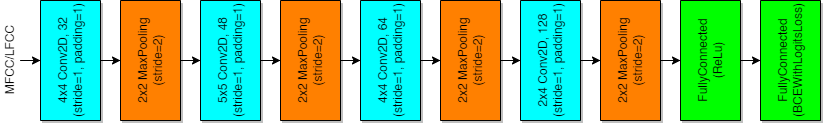
\includegraphics[width=\textwidth]{cnn.png}
    \caption{Shallow CNN Architecture.}
    \label{fig:shallow_cnn_architecture}
\end{figure}

The proposed shallow CNN architecture takes as input the 2D representation of the audio signal $\overbar{\mathbf{X}}_w$ (either MFCC or LFCC) and outputs a single-element vector indicating the likelihood of the analyzed audio belonging to each class. The architecture, as shown in Figure ~\ref{fig:shallow_cnn_architecture}, is composed of four 2D convolutional layers, each one followed by a max-pooling layer ($2 \times 2$ pool size and $2 \times 2$ stride). The first and third convolutional layers are composed of 32 and 64 filters with size $4 \times 4$, respectively. The second convolutional layer consists of 48 filters with size $5 \times 5$. The last convolutional layer is composed of 128 filters with size $2 \times 4$. All the four convolutional layers have stride size $1 \times 1$ and padding size $1 \times 1$. The final convolutional layer is then flattened and connected to a fully connected layer with the ReLu activation function outputting a 128-element vector. A last fully connected layer outputs a 1-element vector used to get the final binary classification result, i.e., human or bot. A label of 0 would imply that the audio signal is classified as fake (generated by a bot), while a label of 1 would imply that the audio signal is classified as real (generated by a real human).

\subsection{Time-Domain Synthetic Speech Detection}

Hua et al. \cite{Hua_2021} proposed Time-Domain Synthetic Speech Detection (TSSD), an end-to-end synthetic speech detection framework that uses deep neural networks (DNN) for feature extraction as well as classification. This lightweight neural network takes in raw audio waveforms without any pre-transforms or hand-crafted feature engineering. Its architecture is described in Figure \ref{fig:tssd_archi}. The first block is a 1x7 1D convolutional layer with 16 channels, followed by Batch Normalization (BN), ReLU activation and max-pooling with kernel size 4. Next, ResNet-style modules \cite{He2016DeepRL} are stacked $M$ times (in our network, $M$ = 4) with a max-pool layer of kernel size 4. Each of these modules has 3 1x3 convolution layers whose output is concatenated with the original input transformed by a 1x1 convolution (i.e., a skip connection), with BN and ReLU applied at the end of each of these layers. In our model, $C_R$, the number of channels, is 16 for the first ResNet block, 32 for the second, 64 for the third and 128 for the last. Finally, this is followed by 3 fully connected layers (where $C_L$, the output dimension, is 128 for the first linear layer, 64 for the second, and 32 for the last) and the output is produced by a softmax layer.

\begin{figure}[htbp]
    \centering
    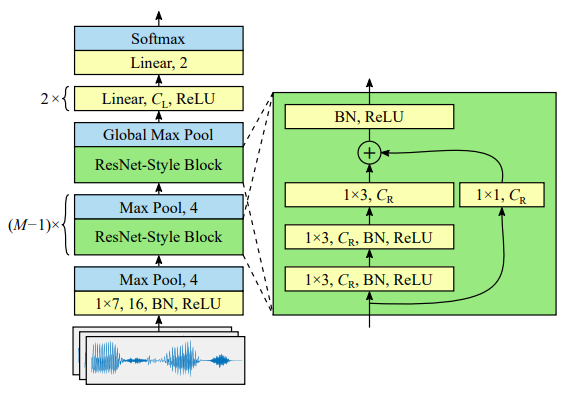
\includegraphics[width=\textwidth]{tssd.png}
    \caption{TSSD Architecture.}
    \label{fig:tssd_archi}
\end{figure}

%%%%%%%%%%%%%%%%%%%%%%%%%%%%%%%%%%%%%%%%%%%%%%%%%%%%%%%%%%%%%%%%%%%%%%%%%%%%%%%
%% Experiments
\section{Experiments and Result}

\textbf{Training and Testing Setup.} We choose to conduct experiments using the two most challenging experiment setups described in WaveFake \cite{frank2021wavefake}.
\begin{itemize}
    \item \textbf{In-distribution Setup}: We use 80\% MelGAN + 80\% LJSpeech for training, and 20\% MelGAN + 20\% LJSpeech for testing. i.e., the Real-to-Fake ratio in training is 1:1.
    \item \textbf{Out-of-distribution Setup}: We use everything except MelGAN + 80\% LJSpeech for training, and 20\% MelGAN + 20\% LJSpeech for testing. i.e., the Real-to-Fake ratio in training is roughly 7.4:1.
\end{itemize}
\textbf{Loss Function.} We use the Binary Cross Entropy Loss (BCELoss) as the training loss for this binary classification problem. In particular, we use the  \textcolor{blue}{\texttt{torch.nn.BCEWithLogitsLoss}} function from PyTorch \cite{NEURIPS2019_9015}, which combines the Sigmoid function with the BCELoss in a single layer to achieve better numerical stability. When the model is trained in the out-of-distribution setting, we calculate the ratio of the number of positive samples to the number of negative samples, i.e. pos\_weight, and use this as the additional weight for the loss. By doing so, the loss acts as if there are an equal amount of positive and negative samples.

\begin{equation}
    l_n = - w_n \left[ y_n \cdot \log \sigma(x_n) + (1 - y_n) \cdot \log (1 - \sigma(x_n)) \right]
\end{equation}
\begin{equation}
    \ell(x, y) = mean(L) = mean(\{l_1,\dots,l_N\}^\top)
\end{equation}

\textbf{Hyper-parameters.} For most of the experiments, models are trained on a single NVIDIA RTX 3090 graphics processing unit with a batch size of 256. We use the Adam \cite{Adam} algorithm with an initial learning rate of $0.0005$ and a weight decay of $0.0001$ for stochastic optimization.

\textbf{Evaluation Metrics.} In Table~\ref{tab:eer}, we follow WaveFake \cite{frank2021wavefake} to report the Equal Error Rate (EER) (a.k.a. Crossover Error Rate), which is commonly used to measure the overall accuracy of a biometric system. EER is defined as the common value where the False Positive Rate (FPR) equals the False Negative Rate (FNR). Lower EER values indicate better performance. Additionally, in Table~\ref{table:f1_auc}, we also report the F1 score (a.k.a. balanced F-score) and the Area Under the Receiver Operating Characteristic Curve (ROC AUC). Higher F1 score and larger AUC indicate better performance.

\begin{table}[h!]
    \centering
    \caption{Experimental Results Reported in EER}
    \begin{tabular}{lcc}
        \toprule
        Model (input feature type)                               & In-dist Setup    & Out-of-dist Setup \\ \midrule
        \rule{0pt}{2.4ex} GMM (w/ LFCC) \cite{frank2021wavefake} & $0.148$          & $0.220$           \\
        \rule{0pt}{2.4ex} RawNet2 (w/ wave) \cite{RawNet2}       & $0.001$          & $\mathbf{0.008}$  \\ \midrule
        \rule{0pt}{2.4ex} VanillaRNN (w/ wave)                   & $0.350$          & $--$              \\
        \rule{0pt}{2.4ex} Bi-LSTM (w/ wave)                      & $0.264$          & $--$              \\
        \rule{0pt}{2.4ex} Bi-LSTM (w/ MFCC)                      & $0.040$          & $--$              \\
        \rule{0pt}{2.4ex} Bi-LSTM (w/ LFCC)                      & $0.004$          & $\mathbf{0.044}$  \\
        \rule{0pt}{2.4ex} ShallowCNN (w/ MFCC)                   & $0.004$          & $--$              \\
        \rule{0pt}{2.4ex} ShallowCNN (w/ LFCC)                   & $\mathbf{0.000}$ & $0.093$           \\
        \rule{0pt}{2.4ex} TSSD (w/ wave)                         & $0.001$          & $0.056$           \\
        % \rule{0pt}{2.4ex} GMM using SGD (w/ MFCC)                & $0.280$          & $--$              \\
        \bottomrule
    \end{tabular}
    \begin{flushleft}
        \scriptsize{GMM (w/ LFCC) and RawNet2 (w/ wave) results are provided by WaveFake \cite{frank2021wavefake}. We round all results to three decimal places following \cite{frank2021wavefake}, hence, $0.000$ implies the actual value is less than $0.0005$. The dashed line indicates that the experiment was not performed due to time constraints.}
    \end{flushleft}
    \vspace{-1em}
    \label{tab:eer}
\end{table}

\begin{table}[h!]
    \centering
    \vspace{2em}
    \caption{Experimental Results Reported in F1 Score and AUC}
    \begin{tabular}{lcccc}
        \toprule
                                               & \multicolumn{2}{c}{In-dist Setup} & \multicolumn{2}{c}{Out-of-dist Setup}                                        \\
        \cmidrule{2-3}                            \cmidrule{4-5} \rule{0pt}{2.2ex}
        Model (input feature type)             & F1-score                          & ROC AUC                               & F1-score         & ROC AUC           \\ \midrule
        \rule{0pt}{2.4ex} VanillaRNN (w/ wave) & $0.649$                           & $0.653$                               & $--$             & $--$              \\
        \rule{0pt}{2.4ex} Bi-LSTM (w/ wave)    & $0.742$                           & $0.750$                               & $--$             & $--$              \\
        \rule{0pt}{2.4ex} Bi-LSTM (w/ MFCC)    & $0.960$                           & $0.960$                               & $--$             & $--$              \\
        \rule{0pt}{2.4ex} Bi-LSTM (w/ LFCC)    & $0.996$                           & $0.996$                               & $\mathbf{0.965}$ & $\mathbf{0.9651}$ \\
        \rule{0pt}{2.4ex} ShallowCNN (w/ MFCC) & $0.997$                           & $0.997$                               & $--$             & $--$              \\
        \rule{0pt}{2.4ex} ShallowCNN (w/ LFCC) & $\mathbf{1.000}$                  & $\mathbf{1.000}$                      & $0.939$          & $0.937$           \\
        \rule{0pt}{2.4ex} TSSD (w/ wave)       & $0.999$                           & $0.999$                               & $0.957$          & $0.956$           \\
        % \rule{0pt}{2.4ex} GMM using SGD (w/ MFCC) & $0.780$                           & $0.780$                               & $--$             & $--$              \\
        \bottomrule
    \end{tabular}
    \begin{flushleft}
        \scriptsize{GMM (w/ LFCC) and RawNet2 (w/ wave)'s F1 and AUC results are not reported by WaveFake \cite{frank2021wavefake}. We round all results to three decimal places, hence, $1.000$ implies the actual value is larger than or equal to $0.9995$. The dashed line indicates that the experiment was not performed due to time constraints.}
    \end{flushleft}
    \vspace{-1em}
    \label{table:f1_auc}
\end{table}

%%%%%%%%%%%%%%%%%%%%%%%%%%%%%%%%%%%%%%%%%%%%%%%%%%%%%%%%%%%%%%%%%%%%%%%%%%%%%%%
%% Analysis

\section{Analysis}
We expect the models trained with the out-of-distribution setup to take significantly more time during training, and this was indeed the case. However, in terms of performance, both models trained with the in-distribution setup and the out-of-distribution setup performed similarly well.

Two anomalous data points of interest that we can manually inspect further are \emph{LJ048-0107} and \emph{LJ050-0267}. Five of our classifier models wrongly predicted the categories of those two data points. More specifically, \emph{LJ048-0107} was wrongly classified by \emph{ShallowCNN\_lfcc\_O}, \emph{SimpleLSTM\_mfcc\_I}, \emph{TSSD\_wave\_I}, \emph{WaveLSTM\_wave\_I}, and \emph{WaveRNN\_wave\_I}, while \emph{LJ050-0267} was wrongly classified by \emph{ShallowCNN\_lfcc\_O}, \emph{ShallowCNN\_mfcc\_I}, \emph{SimpleLSTM\_mfcc\_I}, \emph{WaveLSTM\_wave\_I}, and \emph{WaveRNN\_wave\_I}.

A more interactive and exploratory version of this qualitative analysis is provided here: \url{https://markhh.com/AudioDeepFakeDetection}

As demonstrated on the aforementioned interactive GUI page, all of the features of \emph{LJ048-0107} and \emph{LJ050-0267} that we have used for our models are quite similar. The main blocks in each of the features are mostly the same, and they only differ in the finer details. Therefore, this explains why the models have a harder time in differentiating them.

%%%%%%%%%%%%%%%%%%%%%%%%%%%%%%%%%%%%%%%%%%%%%%%%%%%%%%%%%%%%%%%%%%%%%%%%%%%%%%%
%% Conclusion
\section{Conclusion}
In this project, we implemented, tested, and compared several deep learning architectures to classify human and bot speech with the WaveFake and LJSpeech datasets as the common benchmark in an attempt to measure their performance. From our results, we conclude that while the various networks included in this research are able to perform relatively well even for data generated by very strong GANs, there are still certain audio data inputs that potential adversaries can craft to fool these networks, such as the ones demonstrated in our analysis. As such, further improvement can still be made to increase the detection strength of these models. The results of this research will be useful in dealing with potential new privacy and security issues due to automatic speech and deepfake voice generation tools. We hope that the achieved results will inspire the research community to further investigate this deepfake detection issue in the near future.

\section*{Acknowledgments}
We would like to thank our course instructors, Dr Matthieu De Mari and Prof Berrak Sisman, for the opportunity to conduct this project. Additionally, we would also like to thank Prof Liu Jun for providing the GPU workstations for this project to conduct experiments.

%%%%%%%%%%%%%%%%%%%%%%%%%%%%%%%%%%%%%%%%%%%%%%%%%%%%%%%%%%%%%%%%%%%%%%%%%%%%%%%
%% Bibliography
\bibliographystyle{unsrt}
\bibliography{references}

\end{document}
